\begin{frame}
	\frametitle{Material}
	
	Material para armar estas slides:
	\begin{itemize}
		\item Cyrill Stachniss - Robot Motion Planning using A*: \url{https://youtu.be/HR1TNa8Lp7w}
		\item Wolfram Burgard - Path and Motion Planning \url{http://ais.informatik.uni-freiburg.de/teaching/ss18/robotics/slides/19-pathplanning-long.pdf}
		\url{http://ais.informatik.uni-freiburg.de/teaching/ss16/robotics/recordings/19-path-and-motion-planning-part1.mp4}
		\url{http://ais.informatik.uni-freiburg.de/teaching/ss16/robotics/recordings/19-path-and-motion-planning-part2.mp4}
		\url{http://ais.informatik.uni-freiburg.de/teaching/ss16/robotics/recordings/19-path-and-motion-planning-part3.mp4}
	\end{itemize}
	
\end{frame}

\begin{frame}
	\frametitle{Motion Planning}
	\note{Información extraída de http://ais.informatik.uni-freiburg.de/teaching/ss18/robotics/slides/19-pathplanning-long.pdf}
	
	Latombe (1991): ``... eminently necessary since, by definition, a robot accomplishes tasks by moving in the real world.''
	
	Objetivos:
	\begin{itemize}
		\item Trayectorias sin colisiones.
		\item El robot debe llegar a la ubicación de destino lo más rápido posible.
	\end{itemize}
\end{frame}

\begin{frame}
	\frametitle{Desafíos}
	\note{Información extraída de http://ais.informatik.uni-freiburg.de/teaching/ss18/robotics/slides/19-pathplanning-long.pdf}
	
	\begin{itemize}
		\item Calcular el camino óptimo considerando potenciales incertidumbres en las acciones
		\item Generar rápidamente acciones en el caso de objetos imprevistos
	\end{itemize}
	
\end{frame}


\begin{frame}
	\frametitle{Arquitectura clásica}
	\note{Información extraída de http://ais.informatik.uni-freiburg.de/teaching/ss18/robotics/slides/19-pathplanning-long.pdf}
	
	\begin{figure}[!h]
		\includegraphics[width=0.8\textwidth]{images/path_planning_architecture.pdf}
	\end{figure}
	
\end{frame}

\begin{frame}
    \frametitle{Arquitectura clásica}
    \note{Información extraída de slides Martin Saska}
    
    \begin{figure}[!h]
        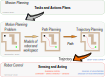
\includegraphics[width=0.5\textwidth]{images/motion_planning_architecture.pdf}
    \end{figure}

    {\bf Motion planning} es parte del ciclo de {\bf mission planning}. Los algoritmos offline se convierten en planificaciones online.
    
\end{frame}


\begin{frame}
	\frametitle{Dynamic Window Approach}
	\note{Información extraída de http://ais.informatik.uni-freiburg.de/teaching/ss18/robotics/slides/19-pathplanning-long.pdf}
	
	
	\TODO{Completar con slides: \url{http://ais.informatik.uni-freiburg.de/teaching/ss18/robotics/slides/19-pathplanning-long.pdf}}
	
	
\end{frame}

\begin{frame}
	\frametitle{Formulación de Motion Planning}
	\note{Información extraída de http://ais.informatik.uni-freiburg.de/teaching/ss18/robotics/slides/19-pathplanning-long.pdf}

	\begin{itemize}
		\item El {\bf problema de la planificación del movimiento} se puede declarar de la siguiente manera. Dado:
		\begin{itemize}
			\item Una pose inicial del robot
			\item Una pose final deseada
			\item Una descripción geométrica del robot
			\item Una representación geométrica del entorno
		\end{itemize}
		\item Encontrar un camino que conduzca al robot gradualmente desde el punto de inicio al punto final sin tocar los obstáculos
	\end{itemize}
\end{frame}

\begin{frame}
	\frametitle{Espacio de configuraciones}
	
	\begin{itemize}
		\item Aunque el problema de planificación de movimiento es 		definido en el mundo regular, vive en otro espacio: el {\bf espacio de configuración}
		\item Una configuración de robot q es una especificación de las posiciones de todos los puntos del robot en relación con un sistema de coordenadas fijo
		\item Por lo general, una configuración se expresa como un vector de posiciones y orientaciones
	\end{itemize}

	
\end{frame}

\begin{frame}
	\frametitle{Espacio de configuraciones}
	\begin{itemize}
		\item Hay dos tipos de regiones: libres u ocupadas (con obstáculos)
		\item Sea $\workSpace = \mathbb{R}^{m}$ el \emph{work space} (para un mundo 2D, $\workSpace = \mathbb{R}^{2}$), $\obstaclesSet \in \workSpace$ el conjunto de obstáculos, $\robotInConfiguration(\robotConfiguration)$ en la configuración $\robotConfiguration \in \configurationSpace$.
        La configuración del robot especifica completamente la pose del robot en $\workSpace$ incluyendo la especificación de todos los grados de libertad. (E.g., un robot con un cuerpo rígido en el plano $\configurationSpace = \begin{bmatrix}
            x & y & \theta
        \end{bmatrix} = \mathbb{R}^{2} \times S_{1}$ .)
        
		\begin{align*}
			 \freeConfigurationSpace &= \left\lbrace \robotConfiguration \in \configurationSpace | \robotInConfiguration(\robotConfiguration) \cap \obstaclesSet =  \emptyset \right\rbrace\\
			 \goalConfiguration &= \configurationSpace / \freeConfigurationSpace
		\end{align*}
	
		\item Definimos:\\
		$\startConfiguration$: configuración \emph{start}\\
		$\goalConfiguration$: configuración \emph{goal}
	\end{itemize}
	
\end{frame}

\begin{frame}
	\frametitle{Ejemplo de espacio de configuraciones}
	
	\begin{figure}[!h]
		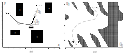
\includegraphics[width=0.8\textwidth]{images/configuration_space_manipulator.pdf}
	\end{figure}
	
\end{frame}

\begin{frame}
    \frametitle{Path vs Trajectory}
    \note{Información extraída de slides Martin Saska}
    
    \begin{itemize}
    \item {\bf Path}: es un mapeo continuo en C-space tal que
        \begin{equation*}
            \continuousPath : [0,1] \rightarrow \freeConfigurationSpace \quad \text{con} \quad \continuousPath(0) = \startConfiguration \quad \text{y} \quad  \continuousPath(1) = \goalConfiguration \quad \text{(\emph{solo hay consideraciones goemétricas})}
        \end{equation*} 
    \item {\bf Trajectory} es un camino con una parametrización explícita del movimiento del robot
    \begin{itemize}
        \item Ejemplo: acompañada por una descripción del las leyes de movimiento del robot
            \begin{equation*}
                \motionLaw : [0, 1] \rightarrow \robotActionSpace,
            \end{equation*}
            donde $\robotActionSpace$ es el espacio de acciones del robot. (\emph{incluye la dinámica del robot})
        \end{itemize}
        \vspace{3em}
        \begin{center}
            \alert{El problema de planeamiento consiste en determinar la función $\continuousPath(.)$}  
        \end{center}
    \end{itemize}
\end{frame}

\begin{frame}
    \frametitle{Problema de Motion Planning}
    \note{Información extraída de slides Martin Saska}
    
    \footnotesize
    
    Teniendo 
    \begin{itemize}
        \item La dinámica de un sistema con estado $\state$ y $\controlCommand$
        \begin{equation*}
            \dfrac{\partial \state}{\partial t} = f(\state,\controlCommand)
        \end{equation*}
        \item Un conjunto de obstáculos $\obstaclesSet \subset \workSpace$ y un conjunto objetivo $\goalSet \subset \workSpace$     
    \end{itemize}
    El problema de Motion Planning consiste en encontrar el comando de control $\controlCommand$ tal que 
    \begin{equation*}
        \state(t) \notin \obstaclesSet \, \text{para} \,  t \in \mathcal{R}_{+} \, \text{y} \, \state(t) \in \goalSet \,  \forall t \ge T_{f} \, \text{para algún finito} \, T_{f} \geq 0,
    \end{equation*}    
    o, retorna que no existe tal señal de control.
    
    \begin{equation*}
        t \in [T_{0} , T_{f}] \rightarrow i \in [0, 1] : \robotConfiguration(t) = \continuousPath(i) \in \freeConfigurationSpace
    \end{equation*}

    Se pueden agregar requerimientos adicionales como
    \begin{itemize}
        \item Suavizado del camino
        \item Restricciones Kinodynamicas\footnote{La planificación kinodinámica se refiere a la tarea de conducir un robot desde un estado inicial hasta un estado objetivo mientras se evaden los obstáculos y se obedecen las restricciones cinemáticas y dinámicas (en resumen, kinodinámicas) que dictan la relación entre los controles del robot y su movimiento.} (\emph{e.g. considerando fuerzas de fricción})
        \item Criterio de Optimalidad (\emph{e.g. shortest vs fastest})
    \end{itemize}
\end{frame}

%\begin{frame}
%	\frametitle{Espacio de configuraciones}
%
%	%Espacio de configuraciones es el estado total del robot y el entorno, incluidas las articulaciones y/o movimiento de ruedas)
%	
%	\begin{figure}[!h]
	%		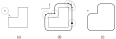
\includegraphics[width=0.8\textwidth]{images/configuration_space_obstacle.pdf}
	%	\end{figure}
%	
%\end{frame}
%
%\begin{frame}
%	\frametitle{Espacio de configuraciones}
%	
%	\begin{figure}[!h]
	%		
\includegraphics[width=0.8\textwidth]{images/workspace_configuration_space.pdf}
	%	\end{figure}
%	
%\end{frame}
%
%
%\begin{frame}
%    \frametitle{Espacio de configuraciones}
%    \note{Información extraída de slides Martin Saska}
%    
%    \begin{figure}[!h]
	%        
\includegraphics[width=0.8\textwidth]{images/workspace_configuration_space.pdf}
	%    \end{figure}
%    
%\end{frame}

\begin{frame}
	\frametitle{Ejemplo de planeamiento sencillo en el C-Space}
	\note{Información extraída de slides Martin Saska}
	
	\begin{figure}
		\subfloat[Problema Motion planning en representación geométrica de $\workSpace$]
		{
			\fbox{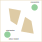
\includegraphics[width=0.33\textwidth]{images/motion_planning_geometrical_example.pdf}}
		}\hspace{1em}
		\subfloat[Problema de Motion planning en representación C-space ]
		{
			\fbox{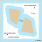
\includegraphics[width=0.33\textwidth]{images/motion_planning_cspace_example.pdf}}
		}
	\end{figure}
	
En este ejemplo, C-space es obtenido por medio de agrandar los obstáculos por el disco $\robotActionSpace$ con radio $\rho$. Aplicando la suma de Minkowski: $\obstaclesSet + \robotActionSpace = \{ x \oplus y | x \in \obstaclesSet, y \in \robotActionSpace \}$
	
\end{frame}

\begin{frame}
	\frametitle{Ejemplo $\obstableConfigurationSpace$ para un robot con rotación}
	\note{Información extraída de slides Martin Saska}
	
	\begin{figure}[!h]
		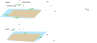
\includegraphics[width=0.6\textwidth]{images/cspace_representation_motivation.pdf}
		\caption{Un simple obstáculo 2D tiene un complicado $\obstableConfigurationSpace$}
	\end{figure}

	\begin{itemize}
		\item Existe un algoritmo determinístico\footnote{J. Canny, PAMI, 8(2):200–209, 1986} pero requiere tiempo exponencial en el número de dimensiones de $\configurationSpace$
		\item Una representación explícita de $\freeConfigurationSpace$ en computacionalmente intratable.
	\end{itemize}
\end{frame}

\begin{frame}
	\frametitle{Representación de C-space}
	\note{Información extraída de slides Martin Saska}
	
	¿Cómo podemos lidiar con una representación continua de C-space?
	
	\begin{figure}[!h]
		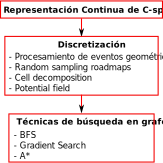
\includegraphics[width=0.4\textwidth]{images/cspace_representation.pdf}
	\end{figure}
	
\end{frame}


\begin{frame}
	\frametitle{Métodos de planning}
	\note{Información extraída de slides Martin Saska}
	
	Algoritmos clásicos de Planeamiento de caminos
	
	\begin{itemize}
		\item Métodos basados en Roadmap (crear un grafo de conectividad del espacio libre)
		\begin{itemize}
			\item Visibility graph
			\item Cell decomposition
			\item Voronoi diagram
		\end{itemize}
		\item Métodos basados en Potential field
	\end{itemize}

	Randomized path/motion planning approaches
	\begin{itemize}
		\item Probabilistic roadmaps (PRM)
		\item Expansive-Spaces Tree (EST)
		\item Rapidly-Exploring Random Tree (RRT) $\leftarrow$ Permite considerar restricciones kinodynamicas.
		\item Optimal sampling based Planner - RRT*
	\end{itemize}
\end{frame}

\begin{frame}
	\frametitle{Visibility Graph}
	\note{Información extraída de slides Martin Saska}
	
	\begin{enumerate}
		\item Computar el visibility graph
		\item Encontrar el camino más corto (e.g. utilizando el algoritmo de Dijkstra)
	\end{enumerate}
	
	\begin{figure}
		\subfloat[Problem]
		{
			
\includegraphics[width=0.2\textwidth]{images/visibility_graph_problem.pdf}
		}\hspace{1em}
		\subfloat[Visibility graph]
		{
			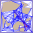
\includegraphics[width=0.2\textwidth]{images/visibility_graph.pdf}
		}\hspace{1em}
		\subfloat[Camino más corto encontrado]
		{
			
\includegraphics[width=0.2\textwidth]{images/visibility_graph_path.pdf}
		}
	\end{figure}

	Construcción del visibility graph:
	\begin{enumerate}
		\item Naïve -- todos los segmentos entre $n$ vértices del mapa $O(n^{3})$
		\item Utilizar árboles de rotación\footnote{M. H. Overmars and E. Welzl, 1988} para un conjunto de segmentos $O(n^{2})$
	\end{enumerate}
	
\end{frame}

\begin{frame}
	\frametitle{Voronoi Diagram}
	\note{Información extraída de slides Martin Saska}
	
	\begin{enumerate}
		\item La hoja de ruta es un diagrama de Voronoi que {\bf maximiza el espacio libre}
		de los obstáculos
		\item Las posiciones de inicio y meta están conectadas al grafo
		\item La ruta se encuentra usando un algoritmo de búsqueda de grafos
	\end{enumerate}
	
	\begin{figure}
		\subfloat[Voronoi diagram]
		{
			
\includegraphics[width=0.2\textwidth]{images/voronoi_diagram_problem.pdf}
		}\hspace{1em}
		\subfloat[Camino en el grafo]
		{
			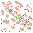
\includegraphics[width=0.2\textwidth]{images/voronoi_diagram.pdf}
		}\hspace{1em}
		\subfloat[Camino encontrado]
		{
			
\includegraphics[width=0.2\textwidth]{images/voronoi_diagram_path.pdf}
		}
	\end{figure}
	
\end{frame}


\begin{frame}
	\frametitle{Visibility Graph vs Voronoi Diagram}
	\note{Información extraída de slides Martin Saska}
	
	\TODO{Completar con slides ECI2015 Martín Saska}
	
\end{frame}

\begin{frame}
	\frametitle{Visibility - Voronoi complex}
	\note{Información extraída de slides Martin Saska}
	
	\TODO{Completar con slides ECI2015 Martín Saska}
	
\end{frame}


\begin{frame}
	\frametitle{Cell Decomposition}
	\note{Información extraída de slides Martin Saska}
	
	\begin{enumerate}
		\item Descomponga el espacio libre en partes. Dos puntos cualesquiera en una región convexa pueden estar directamente conectado por un segmento.
		\item Crear un grafo de adyacencia que represente la conectividad del espacio libre.
		\item Encuentra un camino en el grafo.
	\end{enumerate}
	
	\begin{figure}
		\subfloat[Los centroides reprensetan celdas]
		{
			
\includegraphics[width=0.2\textwidth]{images/cell_decomposition_centroids.pdf}
		}\hspace{1em}
		\subfloat[Conectar celdas adyacentes]
		{
			
\includegraphics[width=0.2\textwidth]{images/cell_decomposition_adjacency_cells.pdf}
		}\hspace{1em}
		\subfloat[Encontrar el camino en el grafo de adyacencia]
		{
			
\includegraphics[width=0.2\textwidth]{images/cell_decomposition_path.pdf}
		}
	\end{figure}
	
\end{frame}


\begin{frame}
	\frametitle{Potential Field}
	
\end{frame}

\begin{frame}
	\frametitle{Randomized Road Maps}
	
\end{frame}

\begin{frame}
	\frametitle{Rapidly Exploring Random Trees (RTTs)}
	\note{Información extraída de slides Martin Saska}
	
	\begin{figure}
		\subfloat[]
		{
			\fbox{
\includegraphics[width=0.3\textwidth]{images/rrt_construction1.pdf}}
		}\hspace{1em}
		\subfloat[]
		{
			\fbox{
\includegraphics[width=0.3\textwidth]{images/rrt_construction2.pdf}}
		}\\
		\subfloat[]
		{
			\fbox{
\includegraphics[width=0.3\textwidth]{images/rrt_construction3.pdf}}
		}\hspace{1em}
		\subfloat[]
		{
			\fbox{
\includegraphics[width=0.3\textwidth]{images/rrt_construction4.pdf}}
		}\\
	\end{figure}
\end{frame}


\begin{frame}
	\frametitle{Sampleo basado en control}
	\note{Información extraída de slides Martin Saska}
	
	\begin{figure}
		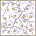
\includegraphics[width=0.5\textwidth]{images/rrt_control_based_sampling.pdf}
	\end{figure}
\end{frame}


\begin{frame}
	\frametitle{Local Path Planning - Bug1}
	\note{Información extraída de slides Martin Saska}

	\begin{itemize}
		\item Rodear el obstáculo para esquivarlo
		\item Cada obstáculo encontrado se rodea completamente una vez, antes de que sea
		dejado en el punto más cercano a la meta
		\item No retorna un camino óptimo; funciona bien con pequeños obstáculos convexos
	\end{itemize}

	\begin{figure}
		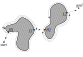
\includegraphics[width=0.6\textwidth]{images/bug1.pdf}
	\end{figure}
\end{frame}

\begin{frame}
	\frametitle{Local Path Planning - Bug2}
	\note{Información extraída de slides Martin Saska}
	
	\begin{itemize}
		\item Rodear el obstáculo siempre por el lado izquierdo o derecho
		\item Dejar el obstáculo si la conexión directa entre inicio y meta se cruzan
	\end{itemize}
	
	\begin{figure}
		
\includegraphics[width=0.7\textwidth]{images/bug2.pdf}
	\end{figure}
	
\end{frame}

\begin{frame}
	\frametitle{Global Planner vs Local Planner}
	
	\begin{figure}[!h]
		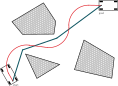
\includegraphics[width=0.5\textwidth]{images/global_local_plan.pdf}
	\end{figure}
	
\end{frame}



\begin{frame}
	\frametitle{Road Map Planning}
	
\end{frame}

\begin{frame}
	\frametitle{Randomized Road Maps}
	
\end{frame}

\begin{frame}
	\frametitle{From Road Maps to Paths}
	
\end{frame}

\begin{frame}
	\frametitle{Randomized Road Maps}
	
\end{frame}

\begin{frame}
	\frametitle{Randomized Road Maps}
	
\end{frame}

\begin{frame}
	\frametitle{Randomized Road Maps}
	
\end{frame}

\begin{frame}
	\frametitle{Markov Decision Process}
	
\end{frame}

